\documentclass{beamer}
\usepackage[utf8]{inputenc}
\usepackage[T1]{fontenc}
\usepackage[french]{babel}

\usepackage{amsmath}
\usepackage{amssymb}
\usepackage{color}
\usepackage{graphicx}
\usepackage[normalem]{ulem}

\newenvironment{mld}
{\par\begin{minipage}{\linewidth}\begin{tabular}{rp{\linewidth}}}
{\end{tabular}\end{minipage}\par}
\newcommand{\relat}[1]{\textsc{#1}}
\newcommand{\attr}[1]{\emph{#1}}
\newcommand{\prim}[1]{\uline{#1}}
\newcommand{\foreign}[1]{\#\textsl{#1}}

\usetheme{CambridgeUS}
\title[Projet de SGBD]{Jeux vidéos}
\author[Les Manchots]{Yvon Garbage, Pierre Lefebvre, Grégoire Pichon}
\institute[ENSEIRB-MATMECA]{ENSEIRB-MATMECA}
\date{\today}
%\date{}

\setbeamercolor{title}{bg=red!65!black,fg=white}

\begin{document}

\setlength{\unitlength}{1cm}

\begin{frame}{Présentation}

\titlepage

\end{frame}

\section*{Introduction}
\begin{frame}
\begin{block}{Sujet}
\begin{center}
Gérer une communauté de joueurs de jeux vidéos. Un ensemble de joueurs doit pouvoir commenter et juger des commentaires sur un ensemble de jeux. Chaque jeu est relatif à un ensemble de catégories et un ensemble de plateformes où il est disponible.
\end{center}
\end{block}

\begin{block}{Objectifs}
\begin{center}
\begin{itemize}
  \item{Modélisation du problème}
  \item{Réalisation de requêtes en SQL}
  \item{Gestion de la cohérence de la base}
\end{itemize}
\end{center}
\end{block}
\end{frame}

\section{Modélisation}
\subsection{Précisions quant au sujet}
\begin{frame}
\begin{block}{Choix effectués}
\begin{center}
\begin{itemize}
\item Un joueur a forcément une catégorie et une plateforme préférées.
\item Un joueur ne peut noter qu'un fois un jeu, pour un plateforme donnée.
\item Un joueur ne peut donner qu'un seul pouce à un commentaire et aucun à un commentaire qu'il a émis.
\item Gestion de la cohérence des dates.
\item Précisions des cardinalités des associations.
\end{itemize}
\end{center}
\end{block}
\end{frame}

\subsection{Modèle conceptuel}
\begin{frame}
\begin{center}
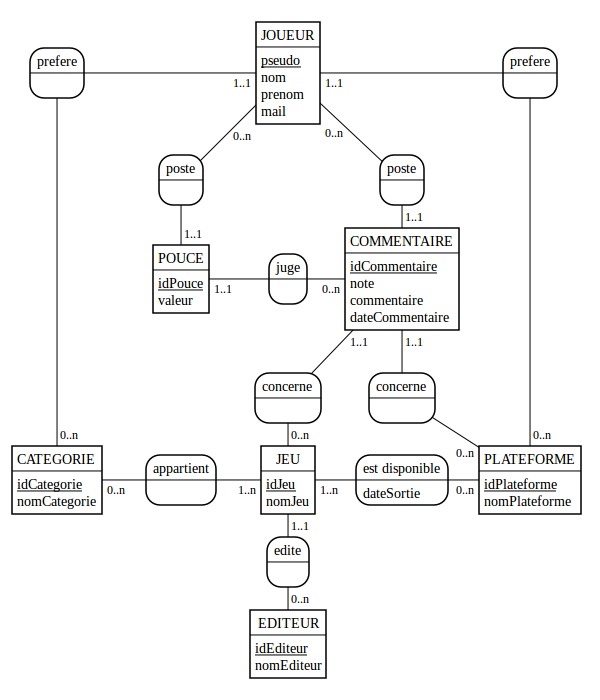
\includegraphics[scale=0.30]{modele_conceptuel.png}
\end{center}
\end{frame}

\subsection{Modèle relationnel}
\begin{frame}
\begin{center}
\begin{mld}
  \relat{Joueur} & (\prim{pseudo}, \attr{nom}, \attr{prenom}, \attr{mail}, \foreign{idCategorie}, \\ 
  \relat{} & \foreign{idPlateforme})\\
  \relat{Pouce} & (\prim{idPouce}, \attr{valeur}, \foreign{pseudo}, \foreign{idCommentaire})\\
  \relat{Commentaire} & (\prim{idCommentaire}, \attr{note}, \attr{commentaire}, \attr{date}, \foreign{pseudo},\\ 
  \relat{} & \foreign{idJeu}, \foreign{idPlateforme})\\
  \relat{Categorie} & (\prim{idCategorie}, \attr{nomCategorie})\\
  \relat{Jeu} & (\prim{idJeu}, \attr{nomJeu}, \foreign{idEditeur})\\
  \relat{Plateforme} & (\prim{idPlateforme}, \attr{nomPlateforme})\\
  \relat{Editeur} & (\prim{idEditeur}, \attr{nomEditeur})\\
  \relat{Appartient} & (\prim{\foreign{idCategorie}, \foreign{idJeu}})\\
  \relat{Est disponible} & (\prim{\foreign{idPlateforme}, \foreign{idJeu}}, \attr{dateSortie})\\ \\
\end{mld}
\end{center}
\end{frame}

\section{Requêtes}
\subsection{Classement des jeux}
\begin{frame}
\begin{center}
SELECT nomJeu AS "Nom du jeu", MP AS "Moyenne pondérée", \\
\ \ \ \ \ \ \ \ \ \ \ \        TotalIC AS "Total des Indices de Confiance des commentaires du jeu" \\
\ \ \ \ \ \ \ \ \ \ \ \ FROM jeu NATURAL JOIN ( \\
\ \ \ \ \ \ \ \ \ \ \ \   SELECT idJeu, ( SUM(note * (1+res.c)/(1+res.d)) ) / ( SUM((1+res.c)/(1+res.d)) ) AS "MP", \\
\ \ \ \ \ \ \ \ \ \ \ \          SUM((1 + res.c)/(1 + res.d)) AS "TotalIC" \\
\ \ \ \ \ \ \ \ \ \ \ \   FROM ( \\
\ \ \ \ \ \ \ \ \ \ \ \      SELECT commentaire.*, \\
\ \ \ \ \ \ \ \ \ \ \ \             SUM(IF(pouce.valeur = '+', 1, 0)) AS "c", SUM(IF(pouce.valeur = '-', 1, 0)) AS "d" \\
\ \ \ \ \ \ \ \ \ \ \ \      FROM commentaire LEFT OUTER JOIN pouce ON commentaire.idCommentaire = pouce.idCommentaire \\
\ \ \ \ \ \ \ \ \ \ \ \      GROUP BY commentaire.idCommentaire) AS res \\
\ \ \ \ \ \ \ \ \ \ \ \   GROUP BY idJeu \\
\ \ \ \ \ \ \ \ \ \ \ \   ORDER BY ( SUM(note * (1+res.c)/(1+res.d)) ) / ( SUM((1+res.c)/(1+res.d)) ) DESC, \\
\ \ \ \ \ \ \ \ \ \ \ \            SUM((1+res.c)/(1+res.d)) DESC) AS classement; \\
\end{center}
\end{frame}

\subsection{Gestion de la cohérence}
\begin{frame}
ALTER TABLE estDisponible ADD CONSTRAINT fk1\_estDisponible \\
\ \ \ \ \ \ \ \ \ \ \ \ FOREIGN KEY (idJeu) \\
\ \ \ \ \ \ \ \ \ \ \ \ REFERENCES jeu (idJeu) ON DELETE CASCADE;
\end{frame}

\section*{Conclusion}
\begin{frame}
\begin{block}{}
\begin{center}
\begin{itemize}
\item Difficulté du choix des contraintes.
\item Plus d'optimisations possibles.
\item Le vrai cas d'étude: la prise en compte des cas d'utilisation.
\end{itemize}
\end{center}
\end{block}
\end{frame}

\end{document}
